\chapter{RISC-V} % Main chapter title
\label{RISC-V} % For referencing the chapter elsewhere, use \ref{Chapter1} 

\section{Einleitung}
\emph{RISC-V} ist eine offene Befehlssatzarchitektur, die 2010 von Entwicklern an der University of California, Berkeley vorgestellt wurde. Sie liegt derzeit in Version 2.1 vor (\textit{Stand: März 2017}). RISC-V basiert auf der RISC (reduced instruction set computing) Design\textit{philosophie}.

\paragraph{RISC.} Die Grundgedanke von RISC-Architekturen ist, dass ein Maschinenbefehl möglichst wenige Taktzyklen in der Ausführung benötigt. Damit grenzt sich RISC zu CISC (complex instruction set computing)-Systemen ab, die komplexe Instruktionen beinhalten und zum Teil viele Taktzyklen zur Ausführung benötigen können. RISC-Programme bestehen daher üblicherweise aus mehr Maschinenbefehlen, die aber tendenziell schneller abgearbeitet werden.

Auch wenn der Begriff \textit{reduced instruction} sich nicht zwangsweise auf die Menge der verfügbaren Maschineninstruktionen bezieht, bestehen RISC-Designs in der Praxis dennoch meist aus weniger Maschinenbefehlen. Außerdem erforden RISC-Architekturen in der Regel eine weniger komplizierte Verschaltung. \footnote{\url{https://www.elektronik-kompendium.de/sites/com/0412281.htm}} Der Vorteil von RISC-Designs ist somit, insbesondere im Hinblick auf dieses Projekt, dass sie einfacher zu implementieren sind.

%----------------------------------------------------------------------------------------
\section{Architektur}
\label{subsec:Register}

\paragraph{Byte Order.} Die RISC-V Architektur verwendet Little-Endian Kodierung.

\paragraph{Speicherarchitektur.} RISC-V ist als \textit{load-store}-Architektur entworfen. Arithmetische und logische Instruktionen greifen daher nicht auf den Speicher zu, stattdessen werden alle Operanden vorher in der Registerbank abgelegt. Operationsergebnisse werden ebenfalls in Registern abgelegt. Speicherzugriffe werden ausschließlich mit \textit{load} bzw. \textit{store}-Befehlen realisiert.

\paragraph{Register.} Die RISC-V Spezifikation definiert $31$ Integer Register $x1 - x31$. Zusätzlich existiert das \textit{zero}-Register $x0$, das eine konstante $0$ beinhaltet. Andere Register (Floating Point) können an dieser Stelle vernachlässigt werden, da sich die umgesetzte CPU auf Integerverarbeitung beschränkt.

\paragraph{Instruktionslänge.} RISC-V Maschinenbefehle sind, wie bei RISC üblich, in einer fixen Länge kodiert. Sie entspricht der Wortbreite der Prozessorarchitektur. Für RISC-V Architekturen sind die Wortbreiten $32, 64$ oder $128$bit vorgesehen.
%----------------------------------------------------------------------------------------

%----------------------------------------------------------------------------------------
\section{RISC-V Varianten}
\label{sec:erweiterung}

\paragraph{Erweiterbarkeit.} Die RISC-V Architektur ist darauf ausgelegt, flexibel erweiterbar zu sein. Die Spezifikation definiert daher mehrere Teilmengen des Befehlssatzes. \cite[p. 4]{RISC}

\paragraph{Mindeststandard.} Um die RISC-V Anforderungen zu erfüllen, muss eine Implementierung zumindest den Basis-Integerbefehlssatz umsetzen (Bezeichnung nach \mbox{RISC-V} Konvention: \textit{I}). Dieser enthält neben Befehlen zur Integerarithmetik auch Integer load- und store-Befehle, sowie die notwendigen Befehle zur Manipulation des Kontrollfluss.

\paragraph{Erweiterungen.} Die allgemeine als \textit{General Purpose} bezeichnete Architektur enthält neben diesem Mindeststandard auch Befehle für Gleitkommaarithmetik (F) mit Double(D) oder Quad-Präzision (Q), für die Handhabung verschiedener Privilegierungen (P), atomare Befehle für die Verwaltung von Nebenläufigkeit (A) und seit der neusten Version 2.1 auch für Bitmanipulation (B), Vectoroperationen (V) und einigen mehr. \cite[p. 4f.]{RISC}

\paragraph{Umgesetzte Instruktionsmenge.} In diesem Projekt wurde sich allerdings darauf beschränkt, eine einfache integerverarbeitende Mikroarchitektur umzusetzen. Als Wortbreite wurden 32bit gewählt. Die Bezeichnung des verwendeten Subsets lautet daher nach RISC-V Konvention \textit{RV32I}. \cite[p. 67ff.]{RISC}
%----------------------------------------------------------------------------------------

%----------------------------------------------------------------------------------------
\section{RV32I}
Das verwendete Subset besteht aus insgesamt $47$ Maschineninstruktionen. Neben Instruktionen zur Integerarithmetik, sind dabei Branch-Instruktionen und Speicherzugriffe enthalten.

\subsection{Instruktionsformate}
RV32I kennt vier verschiedene Typen, in denen Maschineninstruktionen enkodiert sein können: \textit{R-type}, \textit{I-Type}, \textit{S-type} und \textit{U-type} - Befehle, siehe Abbildung \ref{fig:instr_types}. Dabei sind Opcode, sowie Ausgangsregister ($rs1$, $rs2$) und Zielregister ($rd$) der Operationen immer an der gleichen Stelle des Maschinenbefehls kodiert. Sofern ein konstanter Wert (Immediate) in der Instruktion enthalten ist, ist dieser jeweils in den höchstwertigen Bits der Instruktion enkodiert. Diese Einteilung in Instruktionstypen erleichtert die Dekodierung der Instruktionen und führt zu einer simpleren Verschaltung.

\begin{figure} [ht]
  \centering
  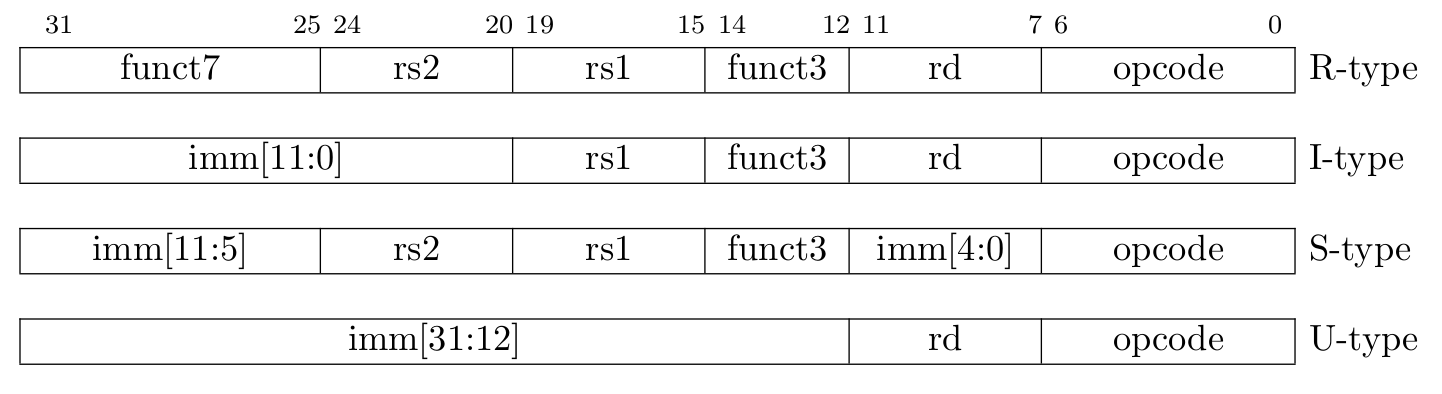
\includegraphics[width=\textwidth]{Figures/instruction_formats}
  \caption{Instruktionsformate. Quelle: \citep[S. 11]{RISC}}
  \label{fig:instr_types}
\end{figure}


\begin{itemize}  
\item Als R-Type sind Register-Instruktionen enkodiert, bei denen beide Operanden in Registern liegen. 
\item Die I-Type-Kodierung ist für Instruktionen vorgesehen, bei denen ein konstanter Wert (\textit{Immediate}) mit einem Wert im Register verrechnet wird.
\item U-Type Befehle sind bedingte und unbedingte Sprungbefehle.
\item Der S-Type wird für schreibende Zugriffe auf den Speicher (store) verwendet. 
\end{itemize}

\subsection{Immediate-Varianten.} Außerdem existieren mehrere Varianten, um Immediates aus den Instruktionen zu Werten zu dekodieren, siehe Abbildung \ref{fig:immediates}. Diese unterschiedlichen Kodierungen sind ebenfalls so gewählt, um die Überschneidungen der einzelnen Formate zu maximieren und dadurch die Implementierung zu vereinfachen. \cite[S. 11f.]{RISC} 

\begin{figure} [ht]
  \centering
  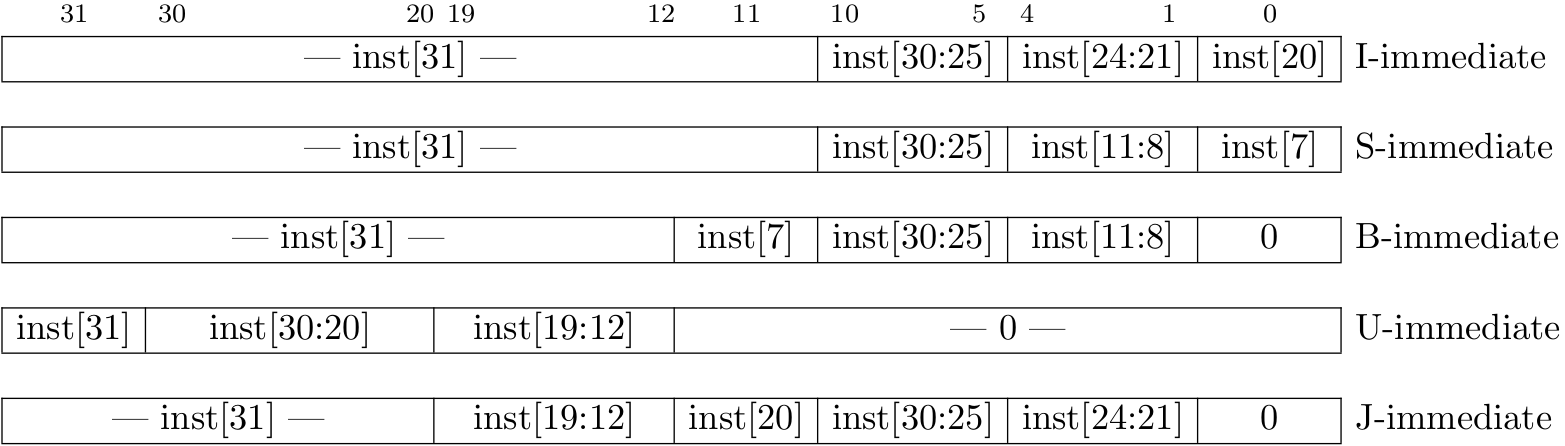
\includegraphics[width=\textwidth]{Figures/immediates}
  \caption{Immediateenkodierungen. Quelle: \citep[S. 12]{RISC}}
  \label{fig:immediates}
\end{figure}

\subsection{Einzelne Instruktionen}
Die in dieser Arbeit umgesetzten Instruktionen des RV32I-Standards können im einzelnen der Tabelle in Anhang \ref{Maschinenbefehle} entnommen werden. Im Folgenden sollen lediglich ein Überblick über Instruktionen geschaffen werden und ein Befehl exemplarisch im Detail dargestellt werden.

\paragraph{Integerarithmetik.}
Integer verarbeitende Instruktionen bestehen aus solchen, die eine Operation auf zwei Registerwerten ausführen (als R-Type kodiert) oder eine Operation auf einem Registerwert und einem Immediate (I-Type) ausführen. Das Operationsergebnis wird jeweils im Zielregister ($rd$) gespeichert.

In \ref{fig:addi} ist exemplarisch der \textit{ADDI}-Befehl zu sehen. Dieser soll einen im Maschinenbefehl kodierten Immediate-Wert mit einem einem Wert in einem bestimmten Register addieren und das Ergebnis anschließend in einem Zielregister speichern.
 
Dafür ist in der Maschineninstruktion der Opcode $0010011$ (bits $6 - 0$) kodiert, der die Information enthält, dass eine Immediateoperation durchgeführt werden soll. Die bits 14-12 kodieren die \textit{funct3}, die die auszuführende Rechenoperation beschreibt (hier: $000$ für die Addition). Ferner ist das Zielregister $rd$, das Ausgangsregister $rs1$ und der Immediate-Wert (bit $31 - 20$) im Maschinenbefehl selbst kodiert.

\begin{figure} [ht]
  \centering
  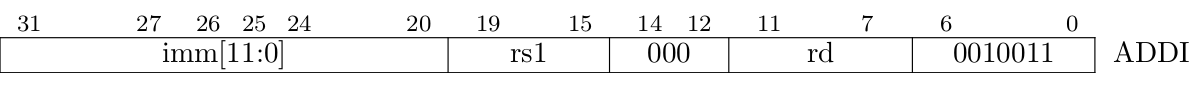
\includegraphics[width=\textwidth]{Figures/ADDI}
  \caption{ADDI-Instruktion.}
  \label{fig:addi}
\end{figure}

In vergleichbarer Weise definiert RISC-V ferner Vergleichsinstruktionen (\textit{SLTI}), logische Operationen (\textit{ANDI, ORI, XORI}) und Shiftoperationen (\textit{SLLLI, SRLI, SRAI}). 

Es ist außerdem der spezielle \textit{LUI}-Befehl vorgesehen, der benötigt wird, um 32bit Konstanten in ein Register zu laden. Aufgrund der festen Instruktionslänge von 32bit kann keine ganze 32bit Immediate in einer Instruktion kodiert werden. \textit{LUI} lädt deshalb nur die ersten 20bit eines Werts und füllt den Rest mit $0$. In einem zweiten Schritt kann dann durch den \textit{ORI} Befehl der restliche Teil geladen werden.

TODO: Register-Register

\paragraph{Kontrollfluss.}
Um die Reihenfolge, mit der die Maschinenbefehle ausgeführt werden zu manipulieren, existieren bedingte (\textit{BEQ, BNE, BLT, BGE}) und unbedingte (\textit{JAL, JALR}) Sprungbefehle.

\paragraph{Speicherzugriffe.}
Da RISC-V als load-store-Architektur entworfen ist, sind Zugriffe auf den Speicher nur in speziellen load/store-Befehlen vorgesehen. Die \textit{load}-Instruktion lädt einen Wert aus dem Speicher in ein Register, die \textit{store}-Instruktion schreibt einen Registerinhalt an eine bestimmte Speicheradresse. RISC-V erlaubt dabei Zugriffe auf Bytes, Halfwords und Words.
%----------------------------------------------------------------------------------------

